%%%%%%%%%%%%%%%%%%%%%%%%%%%%%%%%%%%%%%%%%%%%%%%%%%%%%%%%%%%%%%%%%%%
% CONTROL FLOW MANAGER
%%%%%%%%%%%%%%%%%%%%%%%%%%%%%%%%%%%%%%%%%%%%%%%%%%%%%%%%%%%%%%%%%%%
%
\section{Control Flow Manager}
\label{sec:cfmgr}
%
Harbor needs to manage the control flow within the system for two
reasons.
%
First, the run-time needs to track the identity of the domain
that is currently executing.
%
This information is required to validate memory accesses.
%
Second, the code within the trusted domain, such as the memory map API
needs to be protected from being executed accidentally by other
domains.
%
This is achieved by enforcing restrictions on the control flow within
the system.
%
The \emph{control flow manager} ensures that control can never flow out of
a domain except via calls to functions exported by the kernel or modules in
other domains, and via the corresponding returns.
%
Conversely, control flow can enter a domain only through an exported
function or through the return site of a call that was made to a
function exported by some other domain.
%
These conditions can be verified statically for most cases.
%
However, a user module's control flow might also be affected by internal memory
corruption.
%
Unfortunately, programming errors can cause a module to corrupt its own state, even with
protection domains.
%
%% The protection domains cannot
%% prevent such internal memory corruption.
%
%
For example, function pointers (commonly used to implement callbacks)
are stored in RAM.
%
Return addresses to function call sites are stored in stack.
%
Corruption of these values might cause the processor to execute
arbitrary code, thereby violating the control flow restrictions.
%including the memory map API,
%
%violating one of the requirements of using the memory map for
%protection.
%% ; restricting memory map access to single trusted domain
%% (Refer Section~\ref{subsec:mmap_for_protection}).
%
%
%The control flow manager also tracks the identity of the currently
%executing domain.
%
%This information is required by the memory map checker to validate write
%accesses.
%
The control flow manager enforces the restrictions on control flow
through three main components.
%
\emph{cross domain call} mechanism is used
to transfer control safely from a caller to a callee domain.
%
A corresponding \emph{cross domain return} mechanism restores control back to
a caller domain. 
%
Control flow integrity within a domain is preserved through a \emph{safe stack}
that stores return addresses in protected memory.
%
\emph{Stack Bounds} are used to prevent the corruption of the shared
run-time stack across domains.
%
%==============================================================================
% CROSS DOMAIN CALL
%=============================================================================
\subsection{Cross Domain Call}
\label{sec:crossdomcall}
%
%All function calls made across domains pass through a \textit{cross domain call stub}.
%
%Four operations are performed by the cross domain call stub.
%
%
A cross domain call performs four operations.
%
First, it verifies the call's target address, which
%
should match the address of a function officially \emph{exported} by some
module or the kernel.
%
Second, it saves the caller's domain identity and return address.
%
Third, it sets up a \emph{stack bound}, which prevents the callee from
modifying portions of the stack belonging to the caller.
%
Finally, it jumps to the callee.
%
%% Stack bound is required for run-time stack protection (Section~\ref{subsec:stackguard}).
%
The cross domain call mechanism tries to optimize the performance of these operations.
%

\begin{figure}[htbp]
   \centering
   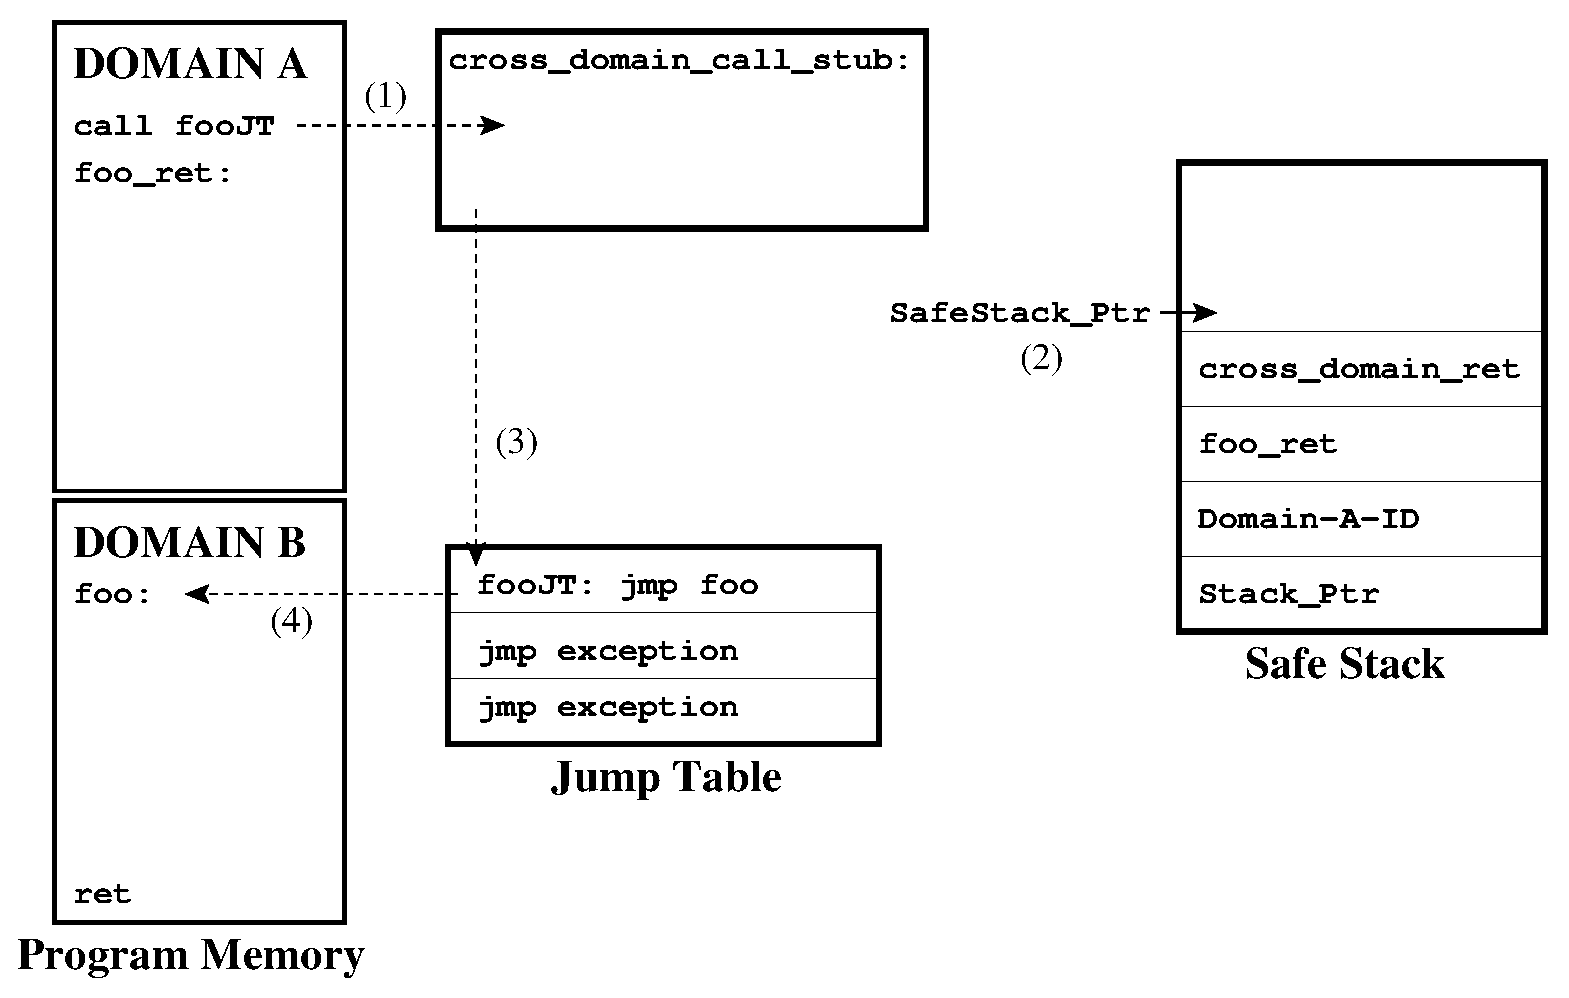
\includegraphics[height=1.5in, keepaspectratio=true]{figures/cross_domain_call_step.eps} 
   \caption[Cross domain call operation]{Cross domain call: (1) All
     cross domain function calls are redirected through the stub. (2)
     The stub stores domain ID, stack bound and return addresses on
     the safe stack. (3) The control flow jumps into an address in
     jump table. (4) The jump table redirects to the call
     implementation in new domain}
   \label{fig:cross_domain_call}
\end{figure}


%
Call address verification is accomplished with the help of a \emph{jump
table}, an extra level of indirection in cross-domain function calls.
%
%% This simplifies the verification of call target addresses
%% and eases the tracking of the system's currently active domain.
%
Modules in a domain are linked with modules in other domains at
load-time as described in Section~\ref{sec:soslinking}.
%
A linker running on the sensor node parses the module's exported functions
and writes them to the jump table.
%
The jump table, which is stored in flash memory, is similar in design
to an interrupt vector table.
%
Each jump table entry is an instruction to jump to an exported
function;
%
the function's address is encoded within the instruction stream.
%
Each domain has its own jump table, containing all the functions exported
by modules in that domain (or, for the kernel domain, all functions
exported by the kernel).
%
Since modules cannot directly write to flash memory, they cannot
corrupt the jump table.
%
Modules that subscribe to functions exported by a particular module
are redirected through the corresponding domain's jump table.
%
This is illustrated in Figure~\ref{fig:cross_domain_call}.
%
%The jump table mechanism is independent of the process used for
%dynamic linking (exporting and subscribing to functions), which might use
%several other techniques~\cite{dunkels06linking}.
%

Each domain is currently allocated one page of internal flash memory for
storing its jump table.
%
%%%% XXX EDDIE STOPS HERE
%
In the AVR architecture, this imposes a limit of 64 exported functions per
domain.
%
The SOS kernel domain exports the system call API that consists of 32
functions.
%
SOS module currently export up to a maximum of 12 functions, allowing
at least 5 modules to share a domain.
%
Empty entries in the jump table are filled with a jump instruction to an
exception routine.
%
All domains' jump table pages are stored contiguously in flash memory,
reducing the overhead of verifying a call's target address and domain.



All function calls made across modules need to pass through a
\textit{cross domain call stub}.
%
This stub, a part of the Harbor runtime, is located
in a trusted region of program memory.
%
In SOS, cross module calls use a macro \texttt{SOS\_CALL};
%
we modified its implementation to force
a call into the cross domain call stub.
%
This is implemented as an assembly routine
within the SOS kernel, with pseudocode
%
shown in
Figure~\ref{fig:cross_domain_call_stub}.
%
\begin{figure} [h]
  \centering
\begin{tiny}
\begin{verbatim}
cross_domain_call_stub(addr_t addr) {
   // Store current return addr in safe stack
   push_ss ret_addr

   // Check if target address is valid
   if (addr > JMP_TBL_BASE) { 
      // Store current state in safe stack
      push_ss curr_domain_id;       
      push_ss curr_stack_bound;
 
      // Compute new domain ID
      curr_domain_id = MSB((addr - JMP_TBL_BASE) << 1);
      if (curr_domain_id > MAX_DOMAIN_ID)
         control_flow_exception();
                 
      // Compute new stack bound (For run-time stack protection)
      curr_statck_bound = STACK_PTR;
     
      // Push the return address of cross domain return
      push_ss cross_domain_return
     
      // Call into jump table
      call addr;
     
cross_domain_return:
      // Restore previous state
      pop_ss curr_stack_bound
      pop_ss curr_domain_id
     
      // Return to caller domain
      ret    
  } else
    control_flow_exception(); 
}
\end{verbatim}
\end{tiny}
\vskip-\baselineskip
  \caption{Pseudocode of Cross Domain Call Stub}
  \label{fig:cross_domain_call_stub}
\end{figure}
%

The stub first stores the return address in the safe stack (Section~\ref{subsec:safe_stack}).
%
%% The design of safe stack is described later in
%% Section~\ref{subsec:safe_stack}.
%
All valid cross-module calls must have target addresses that reside in the
jump table, since
%
modules subscribe to jump table locations
corresponding to the functions exported by other modules.
%
A call into the jump table is checked by a simple compare operation to
the base address of jump table.
%
%% Check against the upper bound of jump table is deferred.
%
The stub then stores the current domain identifier and the stack bound
in the safe stack.
%
A store into the stack is required because cross domain calls can be
chained: domain A calls domain B, which in turn calls domain C.
%
Next, the identity of the callee domain is computed by determining
the jump table page in which the target address falls.
%
%% Jump tables of all domains are organized linearly, starting from the
%% domain 0 jump table located at the base address.
%% %
%% The identifier of target domain can be easily determined by first
%% computing the address offset from the base address of jump table and
%% dividing it by the size of jump table.
%
If the target domain identifier exceeds the maximum number of domains
in the system, then the target address is greater
than the upper bound of jump table; an exception is generated.
%
The callee domain may equal the current domain when a module transfers
control to another module in the same domain.
%
The cross domain return address is pushed to the safe stack, ensuring that
%
control flow will return to the stub.
%
Finally, a call is made into the jump table, which redirects it to the
actual entry point in the target domain.
%
During cross domain return, the previous domain identifier and stack
bound are restored and the control is transferred back to caller
domain.
%

As all domains share a common run-time stack, the cross
domain call stub does not need to copy call arguments.
%
Further, no modifications are made to any data frames set up in the run-time
stack during function calls.
%
Therefore, a single cross domain call and return stub suffices for
all cross domain calls, unlike the per-function stub required by the
original SFI~\cite{wahbe93sfi}.
%
The implementation of the cross domain call stub only uses the
caller-saved registers described by the \texttt{avr-gcc} ABI.
%

The software implementation of Harbor currently disallows all computed
branches except for cross module calls.  
%
This ensures that applications cannot avoid memory and/or control flow
checks, but also prevents certain implementations of control flow
structures like \texttt{switch}.
%
%==============================================================================
% STACK PROTECTION
%==============================================================================
\subsection{Run-Time Stack Protection}
\label{subsec:stackguard}
%
%% Micro-controllers have a single address space and therefore the
%% run-time stack is shared by entire system.
%% %
%% In most architectures, stack is initialized at the end of address
%% space and grows down towards the start of address space.
%% %
%% Run-time stack is used for many purposes.
%% %
%% First, it is used to record return addresses of function calls.
%% %
%% Second, it is used to set up data frames for storing local variables
%% or function arguments that cannot be accommodated in registers.
%% %
%% Third, it is also used to store arguments for variadic functions.
%% %

Harbor shares a common run-time stack across all domains.
%
The design alternative, allocating a private stack per domain,
%
would require too much memory, since stack memory must be allocated
conservatively (the stack can grow significantly during execution).
%
%% Therefore, this design is not feasible on micro-controllers.
%
%% However, stack corruption is a serious problem when it is shared
%% across domains.
%
Harbor implements a \emph{stack bound} to prevent one domain from
corrupting another domain's local variables and other stack
information.
%
The cross domain call stub sets up a stack bound before transferring
control, and the cross domain return stub restores the previous stack
bound.
%
The stack bound is set to the beginning of the callee frame as shown
in the Figure~\ref{fig:stackbound}.
%
As shown in Figure~\ref{fig:checker}, the stack access checker is invoked
for writes to the run-time stack, a statically allocated region of memory
at the high end of the address space.
%
Harbor disallows writes to memory addresses greater than the current stack
bound (assuming a stack that grows down).
%
%% The stack access checker compares the write address to the current stack
%% bound and signals an exception if the address exceeds the stack bound.
%
%% Therefore, a module cannot corrupt the stack belonging to another domain.
%
%% As mentioned in Section~\ref{subsec:cdc}, the current stack bound is
%% updated by the cross domain call and return stubs.
\begin{figure}[htbp]
   \centering
   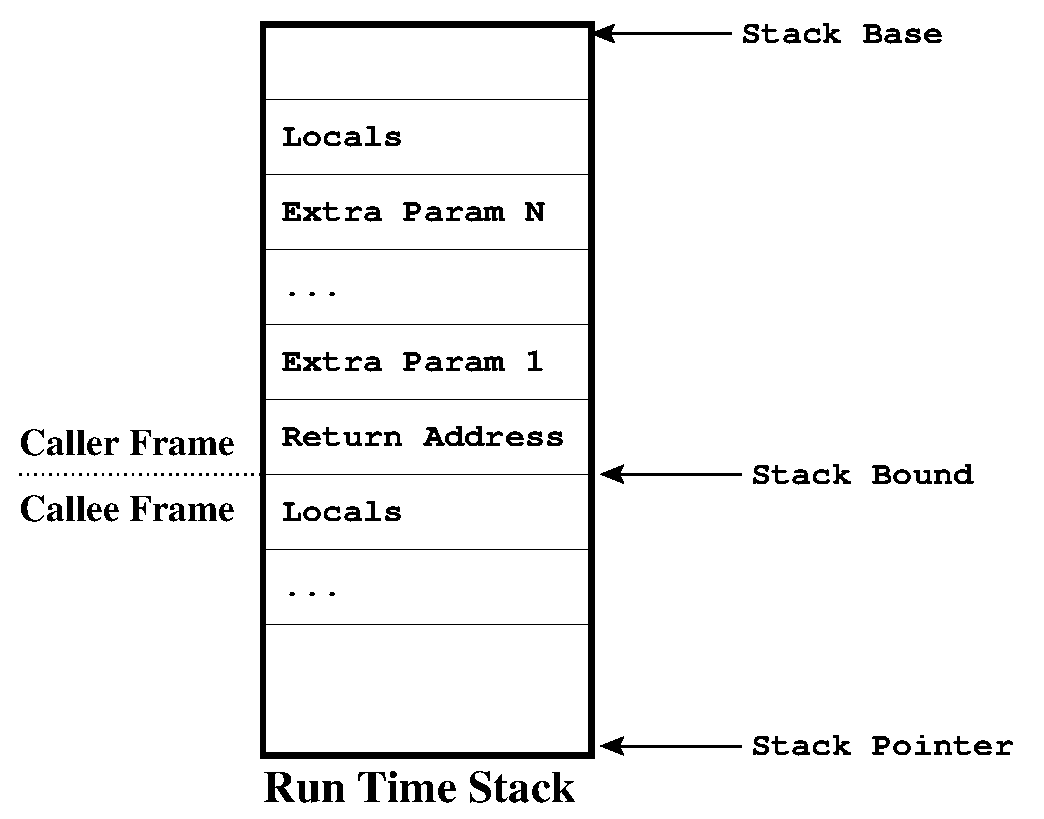
\includegraphics[height=1.5in, keepaspectratio=true]{figures/stack_bounds.eps} 
   \caption[Run-time stack protection using stack bounds]{Run-time stack protection using stack bounds. All writes
     above the current stack bound are disallowed.}
   \label{fig:stackbound}
\end{figure}


The stack bound does prevent cross domain data sharing through the stack,
but we have never encountered an instance of such sharing
in the SOS system.
%


%=============================================================================
% SAFE STACK
%==============================================================================
%
\begin{figure}[htbp]
   \centering
   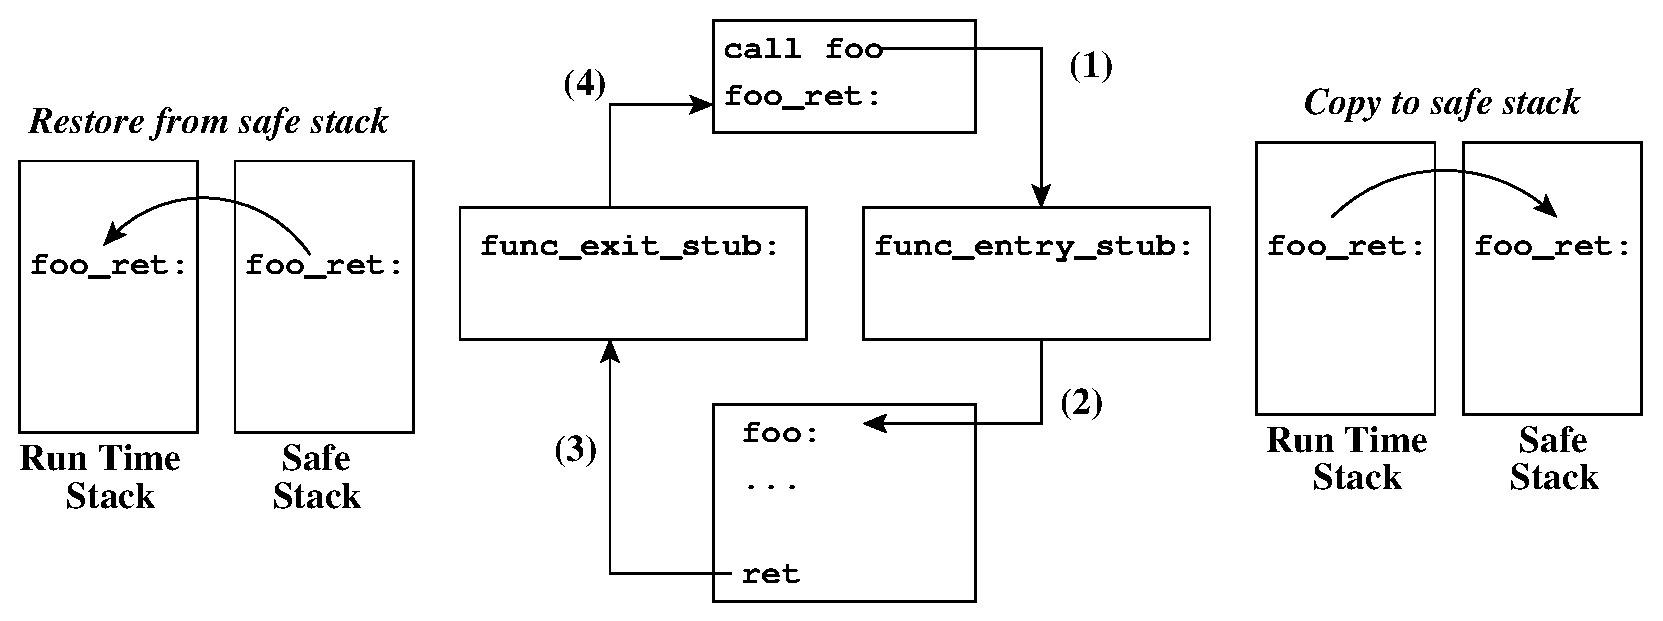
\includegraphics[height=1.5in, keepaspectratio=true]{figures/safe_stack.eps} 
   \caption[Using safe stack for storing return address]{Safe stack
     usage for return address protection. (1) All function calls are redirected
     into the \texttt{func\_entry\_stub}. (2) The stub copies return
     address from run-time stack to safe stack. (3) All returns are
     redirected into the \texttt{func\_exit\_stub}. (4) The stub
     restores copied return address from safe stack to run-time stack.}
   \label{fig:safestack}
\end{figure}
%
\subsection{Safe Stack}
\label{subsec:safe_stack}
%
Correct fault isolation requires that Harbor limit control flow
\emph{within} modules, as well as across modules.
%
A module must not be able to jump into its code arbitrarily, since this
might allow it to avoid a run-time check.
%
The Harbor runtime therefore uses an additional \emph{safe stack}
to preserve the integrity of control flow within and across modules.
%
The safe stack resides in the
trusted domain, preventing any corruption by application wild writes.
%
%% This prevents any corruption to the safe stack caused due to wild
%% writes.
%
%% Only the code executing in the trusted domain can access the safe
%% stack.
%
Harbor stores function calls' return addresses on the safe stack,
protecting them from wild writes by applications in any domain
(Figure~\ref{fig:safestack}).
%
The cross domain call stub also uses the safe stack to store the current
domain ID and run-time stack bound.
%
The safe stack pointer is maintained as a global variable, and manipulated
by sequences of push and pop operations.
%%  is read
%% (and written) before (and after) a sequence of push/pop operations. 
%
%% A module can call any local function within its domain.
%
%% The return addresses of function calls are stored in the run-stack and are
%% protected from corruption from modules in other domains.
%
%% However, a programming error can cause a module to corrupt its own
%% run-time stack.
%
%% This cannot be prevented by protection domains.
%
%% Executing the return instruction on the corrupted run-time stack can cause the
%% control flow to become unpredictable.
%
%% Therefore, Harbor stores all return addresses within the safe stack.
%
A function entry stub, \texttt{func\_entry\_stub}, copies the return
address from the run-time stack onto the safe stack.
%
Similarly, \texttt{func\_exit\_stub} pops the return address from
the safe stack and restores the run-time stack.
%
The entry and exit points of every local function within a domain are
rewritten to invoke these stub routines.
% in the trusted domain that pushes
%(and pops) return addresses into the Safe Stack.
%
%
%Safe Stack is used to overwrite return address values in run-time
%stack.
%
We do not modify the run-time stack in any manner as this would corrupt data
frames setup by functions for storing local data and function
arguments.
%

The safe stack can be placed anywhere in data memory as long as it is
protected from accidental writes and overflow.
%
We usually place the safe stack at the end of all global data in the
system and make it grow upwards.
%
The run-time stack and safe stack thus approach one another.
%
%The software implementation of Harbor does not prevent stack overflow
%corruption.
%
Stack overflow corruption is prevented by checking push operations.

%
%Therefore, all return addresses are checked.
%
%Domains occupy contiguous portions in program memory. 
%
%When the domain is loaded into a system, the Control flow manager records its start and end addresses.
%
%Return addresses are checked to ensure that they lie within bounds of the current domain; else an exception is raised.
%
%Similarly, all computed call addresses are also subject to an identical bounds check.
%
%Calls to static addresses are verified at load time.
%
%All checks are introduced through a binary rewriter.
%\subsection{Summary}
%
Control Flow Manager are a set of components that together ensure that
the memory access checks are not circumvented.
%
It also provides the run-time that tracks the identity of the current
active domain in the system.